\documentclass{beamer}
%\documentclass[pdf]{prosper}
%,colorBG,slideColor
\usepackage{graphicx,color,amsmath,amssymb,amsfonts,amsbsy,amsthm}
\usepackage{verbatim}
\usetheme{Warsaw}
% Node the following tag will orient things right using dvi2pdf.
% Process with LaTeX first, then dvi2pdf.
\special{landscape}
% Fuzz -----------------------------------------------------------
\hfuzz5pt % Don't bother to report overfull boxes < 5pt
% MATH
\newcommand{\includes}{include}
\newcommand{\graphics}{graphics}
\input{\includes/kalman_cmdmaster.tex}
\newtheorem{thm}{Theorem.}
\newtheorem{cor}[thm]{Corollary.}
\newtheorem{con}[thm]{Conjecture.}
\newtheorem{lem}[thm]{Lemma.}
\newtheorem{prop}[thm]{Proposition.}
\newtheorem{defn}[thm]{Definition.}
\renewcommand{\thethm}{}  % unnumbered
\pagestyle{plain}
%%% --------------------------------------------------------------
\begin{document}
% Keep title formatting metadata-safe for current Beamer/hyperref releases.
% The former \vfill/\hrulefill/center construct failed while expanding \maketitle.
\title{\rule{.35\linewidth}{.4pt}\\[1.5ex]
Overview of Kalman Filter Theory and Navigation Applications\\
Day 3}
\author{Michael L. Carroll}
\date{June 16, 2004\\
\vfill \hrulefill \vspace*{.25in} \vfill
{\tiny \textcopyright\ 2004 by Michael L. Carroll}
}
\maketitle
% ----------------------------------------------------------------
\begin{frame}
\textbf{Day 3: Practical Kalman Filtering, Strapdown Navigation and Inertial Error Dynamics\\
Segments}
 \begin{itemize}
 \item Practical Kalman Filtering:  Some Numerical Considerations
 \item The Navigation Problem and Reference Frames
 \item Inertial Error Dynamics
 \item The Basic 9-State Kalman Filter
 \item Challenges of INS Filters
\end{itemize}
\end{frame}
% day2_seg4_numerical/numerical_main.tex
\begin{frame}
  \onslide<1->{
	\frametitle{Some Practical Considerations (Numerical)} 
	\framesubtitle{Topics}
}
\begin{itemize}
  \onslide<2->{
 \item Kalman Filter Theory vs. Reality
}
  \onslide<3->{
 \item Numerical Stability and Round-Off Errors
}
  \onslide<4->{
 \item Matrix Inversion
}
\end{itemize}
\end{frame}
% theory_vs_reality.tex
\begin{frame}
  \onslide<1->{
	\frametitle{Kalman Filter Theory vs. Reality} 
	\framesubtitle{Kalman Assumption Recap}
}
\begin{itemize}
  \onslide<2->{
\item Kalman Assumptions
}
  \onslide<3->{
\begin{itemize}
\item All states linear are modeled correctly
\item Noise parameters are accurately known
\item Initial values are appropriate
\item Process and measurement noise are both Gaussian:  $w\sim\text{N}(0,Q)$, and $v\sim\text{N}(0,R)$
\item Process noise and measurement noise are uncorrelated
\item Measurements are taken at regularly scheduled intervals
\end{itemize} 
}
\end{itemize}
\end{frame}

\begin{frame}
  \onslide<1->{
	\frametitle{Kalman Filter Theory vs. Reality} 
	\framesubtitle{Other Potential Problems}
}
\begin{itemize}
  \onslide<2->{
\item  Continous filters useful for analytical work\\ (e.g., covariance analysis)
}
  \onslide<3->{
\item  But continous filters unrealistic in practice: Always some sort of discretization needed  
}
  \onslide<4->{
\item  Measurements almost never continuous 
}
  \onslide<5->{
\item  Discrete filters acceptable provided continuous estimates are not required 
}
  \onslide<5->{
\item  Suboptimality 
}
\end{itemize}
\end{frame}

\begin{frame}
  \onslide<1->{
	\frametitle{Kalman Filter Theory vs. Reality} 
	\framesubtitle{Sensor Selection}
}
\begin{itemize}
  \onslide<2->{
  \item How do you select appropriate sensors for the problem at hand?
}
  \onslide<3->{
  \item Some obvious general rules:
  \begin{itemize}
	\item The lower the sensor noise characteristics, the more accurate the estimates (narrow sensor noise variance)
}
  \onslide<4->{
    \item The more the merrier, i.e., the more sensors the better\\
	Greater number of lower quality sensors can outperform smaller number of higher quality ones (see kalcompare.m)
}
  \onslide<5->{
    \item Maximize the number of directly observable states
\end{itemize}
}
\end{itemize}
\end{frame}


\begin{frame}
  \onslide<1->{
	\frametitle{Kalman Filter Theory vs. Reality} 
	\framesubtitle{Sensor Selection}
}
\begin{itemize}
  \onslide<2->{
  \item Some less obvious general rules:
}
  \onslide<3->{
  \begin{itemize}
	\item Short-term / long-term complementarity (e.g, GPS vs. INS)
}
  \onslide<4->{
    \item Frequency response of sensor should match that of system
}
  \onslide<5->{
    \item Noise spectrum of sensor should be maximally disjoint from that of system
  \end{itemize}
}
\end{itemize}
\end{frame}

\begin{frame}
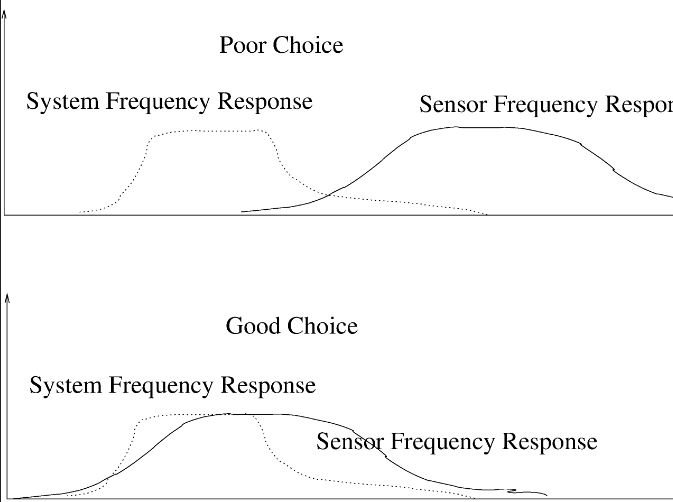
\includegraphics[scale=0.60]{day3_seg1_numerical/sensor_selection.jpg}
\end{frame}

\begin{frame}
  \onslide<1->{
	\frametitle{Kalman Filter Theory vs. Reality} 
	\framesubtitle{}
}
\begin{itemize}
  \onslide<2->{
  \item Choose sensors to match states.\\
E.g., consider the state model
\[
\begin{bmatrix}
\dot{x}_1\\
\dot{x}_2
\end{bmatrix}
= \begin{bmatrix}
0\\
0
\end{bmatrix}
\]
with the measurement model
\[
z = \begin{bmatrix} 1\;\; 0 \end{bmatrix}\begin{bmatrix}
x_1\\
x_2
\end{bmatrix}
+ v
\]
}
  \onslide<3->{
\item   Here $x_1$ is observable but $x_2$ is not, because there are no dynamic paths in $A=I$ flow infomation 
about $x_1$ into $x_2$
}
\end{itemize}
\end{frame}

\begin{frame}
  \onslide<1->{
	\frametitle{Kalman Filter Theory vs. Reality} 
	\framesubtitle{Sensor Selection}
}
\begin{itemize}
  \onslide<2->{
  \item Examine the $H$ matrix that you would use with this sensor!
}
  \onslide<3->{
  \item If it renders some states unobservable, then consider adding 
  additional sensors for those states, or replacing this sensor with one that is more favorable
}
\end{itemize}
\end{frame}
% day3_seg4_ins_challenges/observability.tex
\begin{frame}
  \onslide<1->{
	\frametitle{Observability} 
	\framesubtitle{}
}
\begin{itemize}
  \onslide<2->{
 \item Structural observability is concerned with how $H$ maps measurements into states
}
  \onslide<3->{
  \item Observability means there is a linear path from the measurements to states
}
  \onslide<4->{
  \item Structural observability determined by $\Phi$ and $H$:
}
  \onslide<5->{
\item  If $H$ is $1\times n$, where $n$ is the size of the state vector, then the state $x_0$ 
is said to be \textbf{observable }from $n$ scalar measurements $\set{z_0,\ldots,z_{n-1}}$ if the block matrix
\[
\begin{bmatrix}
H\trans&\Phi\trans H\trans & \cdots & (\Phi\trans)^{n-1}H\trans
\end{bmatrix}
\]
is of rank $n$

}
  \onslide<6->{
 \item Will making measurements as governed by $H$ actually enable us to estimate all of the states 
 in the state vector? 
}
 \end{itemize}
\end{frame}

\begin{frame}
  \onslide<1->{
	\frametitle{Observability} 
	\framesubtitle{Designing Observability into the Filter}
}
\begin{itemize}
  \onslide<2->{
  \item Observability challenge for filters is often a matter of choosing right kinds of sensors
}
  \onslide<3->{
  \item Choosing the right measurement scheduling
}
  \onslide<4->{
  \item Certain kinds of divergence can be the result of poor observability
}
  \onslide<5->{
\item   Example: Let $H=\left[1\;\;0\;\; 0\;\; 0\;\; 0\right]$, 
$\Phi=
\begin{bmatrix}
0&1&0&0&0\\
0&0&1&0&0\\
0&0&0&1&0\\
0&0&0&0&1\\
1& 2&3&4&5
\end{bmatrix}$
}
  \onslide<6->{
	\item What is the rank 
	of $\left[H\trans\;\;\Phi H\trans\;\;\Phi^2 H\trans\;\; \Phi^3 H\trans\;\;\Phi^4 H\trans\right]$?
}
\end{itemize}
\end{frame}



% day2_seg4_numerical/divergence.tex
\begin{frame}
  \onslide<1->{
	\frametitle{Filter Divergence} 
	\framesubtitle{}
}
\begin{itemize}
  \onslide<2->{
\item Kinds of Divergence
}
  \onslide<3->{
\item Causes and Remedies
}
\end{itemize}
\end{frame}

\begin{frame}
  \onslide<1->{
	\frametitle{Filter Divergence} 
	\framesubtitle{Kinds of Divergence}
}
\begin{itemize}
  \onslide<2->{
\item Mean estimation error is supposed to converge to 0
\begin{itemize}
	\item $\esterrdef$
	\item $\expect{\esterr}\rightarrow 0$
	\item Estimate is unbiased: $\expect{\hat{x}(k)}=x(k)$
\end{itemize}
}
  \onslide<3->{
\item Covariance matrix for estimation error is same as state estimation error covariance matrix: $\covmatdef$
}
\end{itemize}
\end{frame}

\begin{frame}
  \onslide<1->{
	\frametitle{Kinds of Divergence} 
	\framesubtitle{}
}
\begin{itemize}
  \onslide<2->{
\item For optimal filter, $P$ will indicate convergence or divergence.
	\begin{itemize}
		\item One common form of divergence due to round-off will send $P$ to zero
	\end{itemize}
}
  \onslide<3->{
\item For suboptimal filters, $P$ will not necessarily indicate divergence
	\begin{itemize}
	  \item $P$ may seem to indicate nominal steady-state values and yet the state estimate may go diverge from the true value
	\end{itemize}
}
\end{itemize}
\end{frame}


\begin{frame}

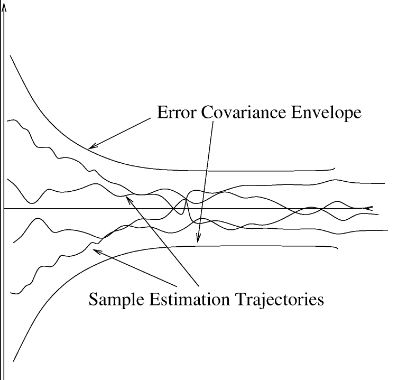
\includegraphics[scale=0.60]{day3_seg1_numerical/covconverge.jpg} 

\end{frame}


\begin{frame}
  \onslide<1->{
	\frametitle{Kinds of Divergence} 
	\framesubtitle{}
}
\begin{itemize}
  \onslide<2->{
\item Going to sleep:  error covariance becomes so small that measurements are no longer believed by the filter
}
  \onslide<3->{
\item Loss of symmetry in $P$
}
  \onslide<4->{
\item Loss of positive definiteness: negative numbers on the diagonal!
}
\end{itemize}
\end{frame}

% day2_seg4_numerical/numstab.tex
\begin{frame}
  \onslide<1->{
	\frametitle{Numerical Stability} 
	\framesubtitle{}
}
\begin{itemize}
  \onslide<2->{
 \item System stability:  Bounded input results in bounded output
}
  \onslide<3->{
 \item Numerical stability: small errors at each computation step do not grow without bound
}
  \onslide<4->{
 \item Matrix Conditioning (will address in discussing SRIF)
}
\end{itemize}
\end{frame}

%\input{day2_seg4_numerical/matrix_conditioning.tex}
% day2_seg4_numerical/roundoff.tex
\begin{frame}
  \onslide<1->{
	\frametitle{Round-Off Errors} 
	\framesubtitle{Joseph Form}
}
\begin{itemize}
  \onslide<2->{
 \item Computer round-off in floating point arithmetic
}
  \onslide<3->{
 \item Unit round-off value is largest number $\eps$ such that $1+\eps=1$
}
  \onslide<4->{
 \item In Matlab, the global symbol "eps" stores the unit round-off value
}
  \onslide<5->{
  \item Round-off errors generally plague the classical covariance update algorithm
\[\covupdateeq\]
\begin{itemize}
  \item Alternative, called the Joseph form, is more robust:
\[\josephcovupdateeq\]
\end{itemize} 
}
\end{itemize}
\end{frame}

\begin{frame}
  \onslide<1->{
	\frametitle{Round-Off Errors} 
	\framesubtitle{De Vries Mechanization}
}
\begin{itemize}
  \onslide<2->{
\item   This form in turn leads to the De Vries mechanization of the
Kalman gain equation.  To see this, first expand
the Joseph form (omitting subscripts for clarity):

}
  \onslide<3->{
\begin{align*}
   P(+)&= P(-)-KHP(-)-P(-)H\trans K\trans+ KHP(-)H\trans K\trans +
   KRK\trans.
\end{align*}
}
\end{itemize}
\end{frame}

\begin{frame}
  \onslide<1->{
	\frametitle{Round-Off} 
	\framesubtitle{De Vries}
}
\begin{itemize}
  \onslide<2->{
\item   Define
\begin{equation}\label{Feq}
  F=PH\trans
\end{equation}
and
\begin{equation}\label{Deq}
  D=HF+R.
\end{equation}

}
  \onslide<3->{
\item   We note that $D$ is symmetric, because
\begin{align*}
  D\trans &= [HF+R]\trans \\
  &= [HPH\trans + R]\trans \\
  &= [HPH\trans] \trans + R\trans \\
  &= [H\trans]\trans P\trans H\trans + R\trans \\
  &= HPH\trans + R & \text{(because $P$ and $R$ are symmetric)}\\
  &= HF + R \\
  &= D.
\end{align*}
}
\end{itemize}
\end{frame}

\begin{frame}
  \onslide<1->{
	\frametitle{Round-Off} 
	\framesubtitle{De Vries}
}
\begin{itemize}
  \onslide<2->{
\item   The gain in standard Kalman gain equation
\[\kalgaineq\] can be written as
\[K=FD^{-1}.\]
}
  \onslide<3->{
\item   Using Eqs.~(\ref{Feq}) and ~(\ref{Deq}), we compute
\begin{align*}
  P(+) &= P(-) - KF\trans - FK\trans + KDK\trans \\
  &= P(-)-K\left[F\trans - \frac{DK\trans}{2} \right] - \left[
  F-\frac{KD}{2}\right]K\trans.
\end{align*}

}
  \onslide<4->{
\item   Letting $G=F-\dfrac{KD}{2}$, we obtain
\begin{equation}\label{dvcovupdateeq}
  \dvcovupdateeq.
\end{equation}

}
\end{itemize}
\end{frame}

\begin{frame}
  \onslide<1->{
	\frametitle{Round-Off} 
	\framesubtitle{De Vries}
}
\begin{itemize}
  \onslide<2->{
\item   The De Vries mechanization implements Eq.~(\ref{dvcovupdateeq}) by
subtracting the $ij^{th}$ element of $GK\trans$ from both the
$ij^{th}$ and $ji^{th}$ elements of $P(-)$. 
}
  \onslide<3->{
\item   The De Vries form of
the covariance update equation is valid for any arbitrary gain
matrix $K$, not just the optimal gains computed from
Eqs.~(\ref{Feq}) and (\ref{Deq}).

}
\end{itemize}
\end{frame}

% day2_seg4_numerical/matinv.tex
\begin{frame}
  \onslide<1->{
	\frametitle{Numerical Stability} 
	\framesubtitle{Matrix Inversion}
}
\begin{itemize}
  \onslide<2->{
 \item Matrix inversion is always risky due to potential ill-conditioning
}
  \onslide<3->{
 \item One way to avoid this is to process measurements sequentially as scalars
}
  \onslide<4->{
 \item Or at least as low-dimensional matrices
}
\end{itemize}
\end{frame}

%% day2_seg4_numerical/symmloss.tex
\begin{frame}
Loss of Symmetry and Positive Definiteness
 \begin{itemize}
 \item
 \item
 \item
\end{itemize}
\end{frame}

% day2_seg4_numerical/exercises.tex
\begin{frame}
  \onslide<1->{
	\frametitle{Exercises} 
}
\begin{itemize}
  \onslide<2->{
\item   1. Let $v=[1\;\; -2]\trans$.  Compute the positive definite, symmetrix matrix $M=vv\trans$

}
  \onslide<3->{
\item   2. Use the following algorithm (Grewal \& Andrews) to factor $M$ into $UDU\trans$ form:
}
\end{itemize}
\end{frame}
\begin{frame}[fragile]
	\frametitle{Exercises} 
\begin{verbatim}
for j=m:-1:1
    for i=j:-1:1
        covar=P(i,j);
        for k=j+1:m
            covar=covar-U(i,k)*D(k,k)*U(j,k);
        end
        if i==j
            D(j,j)=covar;
            U(j,j)=1;
        else
            U(i,j)=covar/D(j,j);
        end
    end
end
\end{verbatim}
\end{frame}


% day3_seg1_navproblem/navproblem_main.tex
\begin{frame}
\textbf{Segment 10\\
The Navigation Problem and Reference Frames\\
Topics}
 \begin{itemize}
 \item Basic Navigation Problem
 \item Earth Referenced Navigation
 \item Coordinate Frame Conversion
 \item Basic Strapdown Navigation Equations
\end{itemize}
\end{frame}
% day3_seg1_navproblem/basicnavprob.tex
\begin{frame}
Basic Navigation Problem
 \begin{itemize}
 \item Where am I?
 \item Where am I headed?
 \item How fast am I going?
\end{itemize}
\end{frame}
\begin{frame}
Basic Navigation Problem
 \begin{itemize}
 \item What's my position?
 \item What's my heading and attitude?
 \item What's my velocity?
\end{itemize}
\end{frame}
\begin{frame}
Solution in Inertial Space
 \begin{itemize}
 \item In inertial space, it's no problem!
 \item Just integrate the acceleration once to get velocity, twice to get
 position.
\[v(T) = v(0) + \int_{0}^{T}\dfrac{d^2r}{dt^2}dt\]
\[r(T) = r(0) + \int_{0}^{T}v(T)dt\]
 \item And integrate the angular rate once to get attitude.
\end{itemize}
\end{frame}

\begin{frame}
Solution in Inertial Space
\begin{itemize}
  \item Solution easy in inertial space because ...
  \begin{itemize}
	\item inertial instruments sense acceleration and rotational rate with respect to inertial coordinate frame 
	\item inertial frame attached to sensor platform
    \item Note: You still need to rotate accelerations from body to inertial coordinates prior to integration (strapdown)
  \end{itemize}
  \item But we don't necessarily want the answer to our questions expressed in terms of inertial coordinates!
\end{itemize} 
\end{frame}

% day3_seg1_navproblem/earthrev.tex
\begin{frame}
Earth Referenced Navigation
 \begin{itemize}
 \item Terrestial navigation seeks to answer nav questions with respect to earth
 \begin{itemize}
   \item Global earth reference
   \item Local or relative navigation
 \end{itemize}
 \item Complications:
 \begin{itemize}
   \item Earth surface is curved (ellipsoid)
   \item Earth is turning (can usually ignore motion about the Sun for terrestrial nav)
 \end{itemize}
\end{itemize}
\end{frame}

% day3_seg1_navproblem/coordconv.tex
\begin{frame}
Coordinate Frames
 \begin{itemize}
 \item Inertial
 \item Earth Fixed
 \item Local Level
 \item Body
\end{itemize}
\end{frame}
\begin{frame}
Coordinate Frames
 \begin{itemize}
  \item Technically speaking, all frames are earth-centered
  \item Practically speaking, we think of the Body frame as centered in the body of the vehicle (usually at center of gravity).
  \item Local Level is thought to be located at surface of earth directly beneath the vehicle.
\end{itemize}
\end{frame}
\begin{frame}
Inertial Reference Frames
 \begin{itemize}
 \item Non-Rotating
 \item Non-Accelerating
 \item Fixed or moving uniformly with respect to another inertial
 frame (fixed stars)
\end{itemize}
\end{frame}
\begin{frame}
Inertial Reference Frames
 \begin{itemize}
 \item Nav problem "easy" in inertial frames
 \item Integrate gyro rates once to get attitude (rotational motion is absolute)
 \item Rotate accelerometer outputs to inertial frame using attitude matrix, then integrate to get inertial
 velocity; integrate velocity to get position.
 \item Would still have to contend with instrument imperfections.
\end{itemize}
\end{frame}
\begin{frame}
Inertial Reference Frame Integrations
\begin{equation}\label{inertacceleq}
\ddot{r}(t)=\specforce+\text{other external forces}
\end{equation}
\begin{equation}\label{inertveleq}
v(T)=\dot{r}(T)=v(0)+\int_{0}^{T}\specforce dt + \int_{0}^{T}(\text{other
external forces})dt
\end{equation}
\begin{equation}\label{inertposeq}
  r(T)=r(0)+\int_{0}^{T}v dt
\end{equation}
\end{frame}
\begin{frame}
Earth Fixed = ECEF = Earth Centered Earth Fixed
 \begin{itemize}
 \item Rotating frame, i.e., non-inertial
 \item Cartesian ($X,Y,Z$ in meters)
 \item Spherical (latitude $\lat$, longitude $\lon$, altitude $\alt$)
 \begin{itemize}
 \item geodetic
 \end{itemize}
\end{itemize}
\end{frame}
\begin{frame}
Local Level
 \begin{itemize}
 \item Tangent to earth's surface but translated to center of
 earth.
 \item Vertical $Z$-axis is normal to earth's surface
 \item $X,Y$-axes are level
 \item Several kinds: $Y$ north-slaved, wander (0 transport rate) or free azimuth
 \item $Y$ makes wander angle $\alpha$ with respect to true north (ENU=East, North, Up).
\end{itemize}
\end{frame}

\begin{frame}
%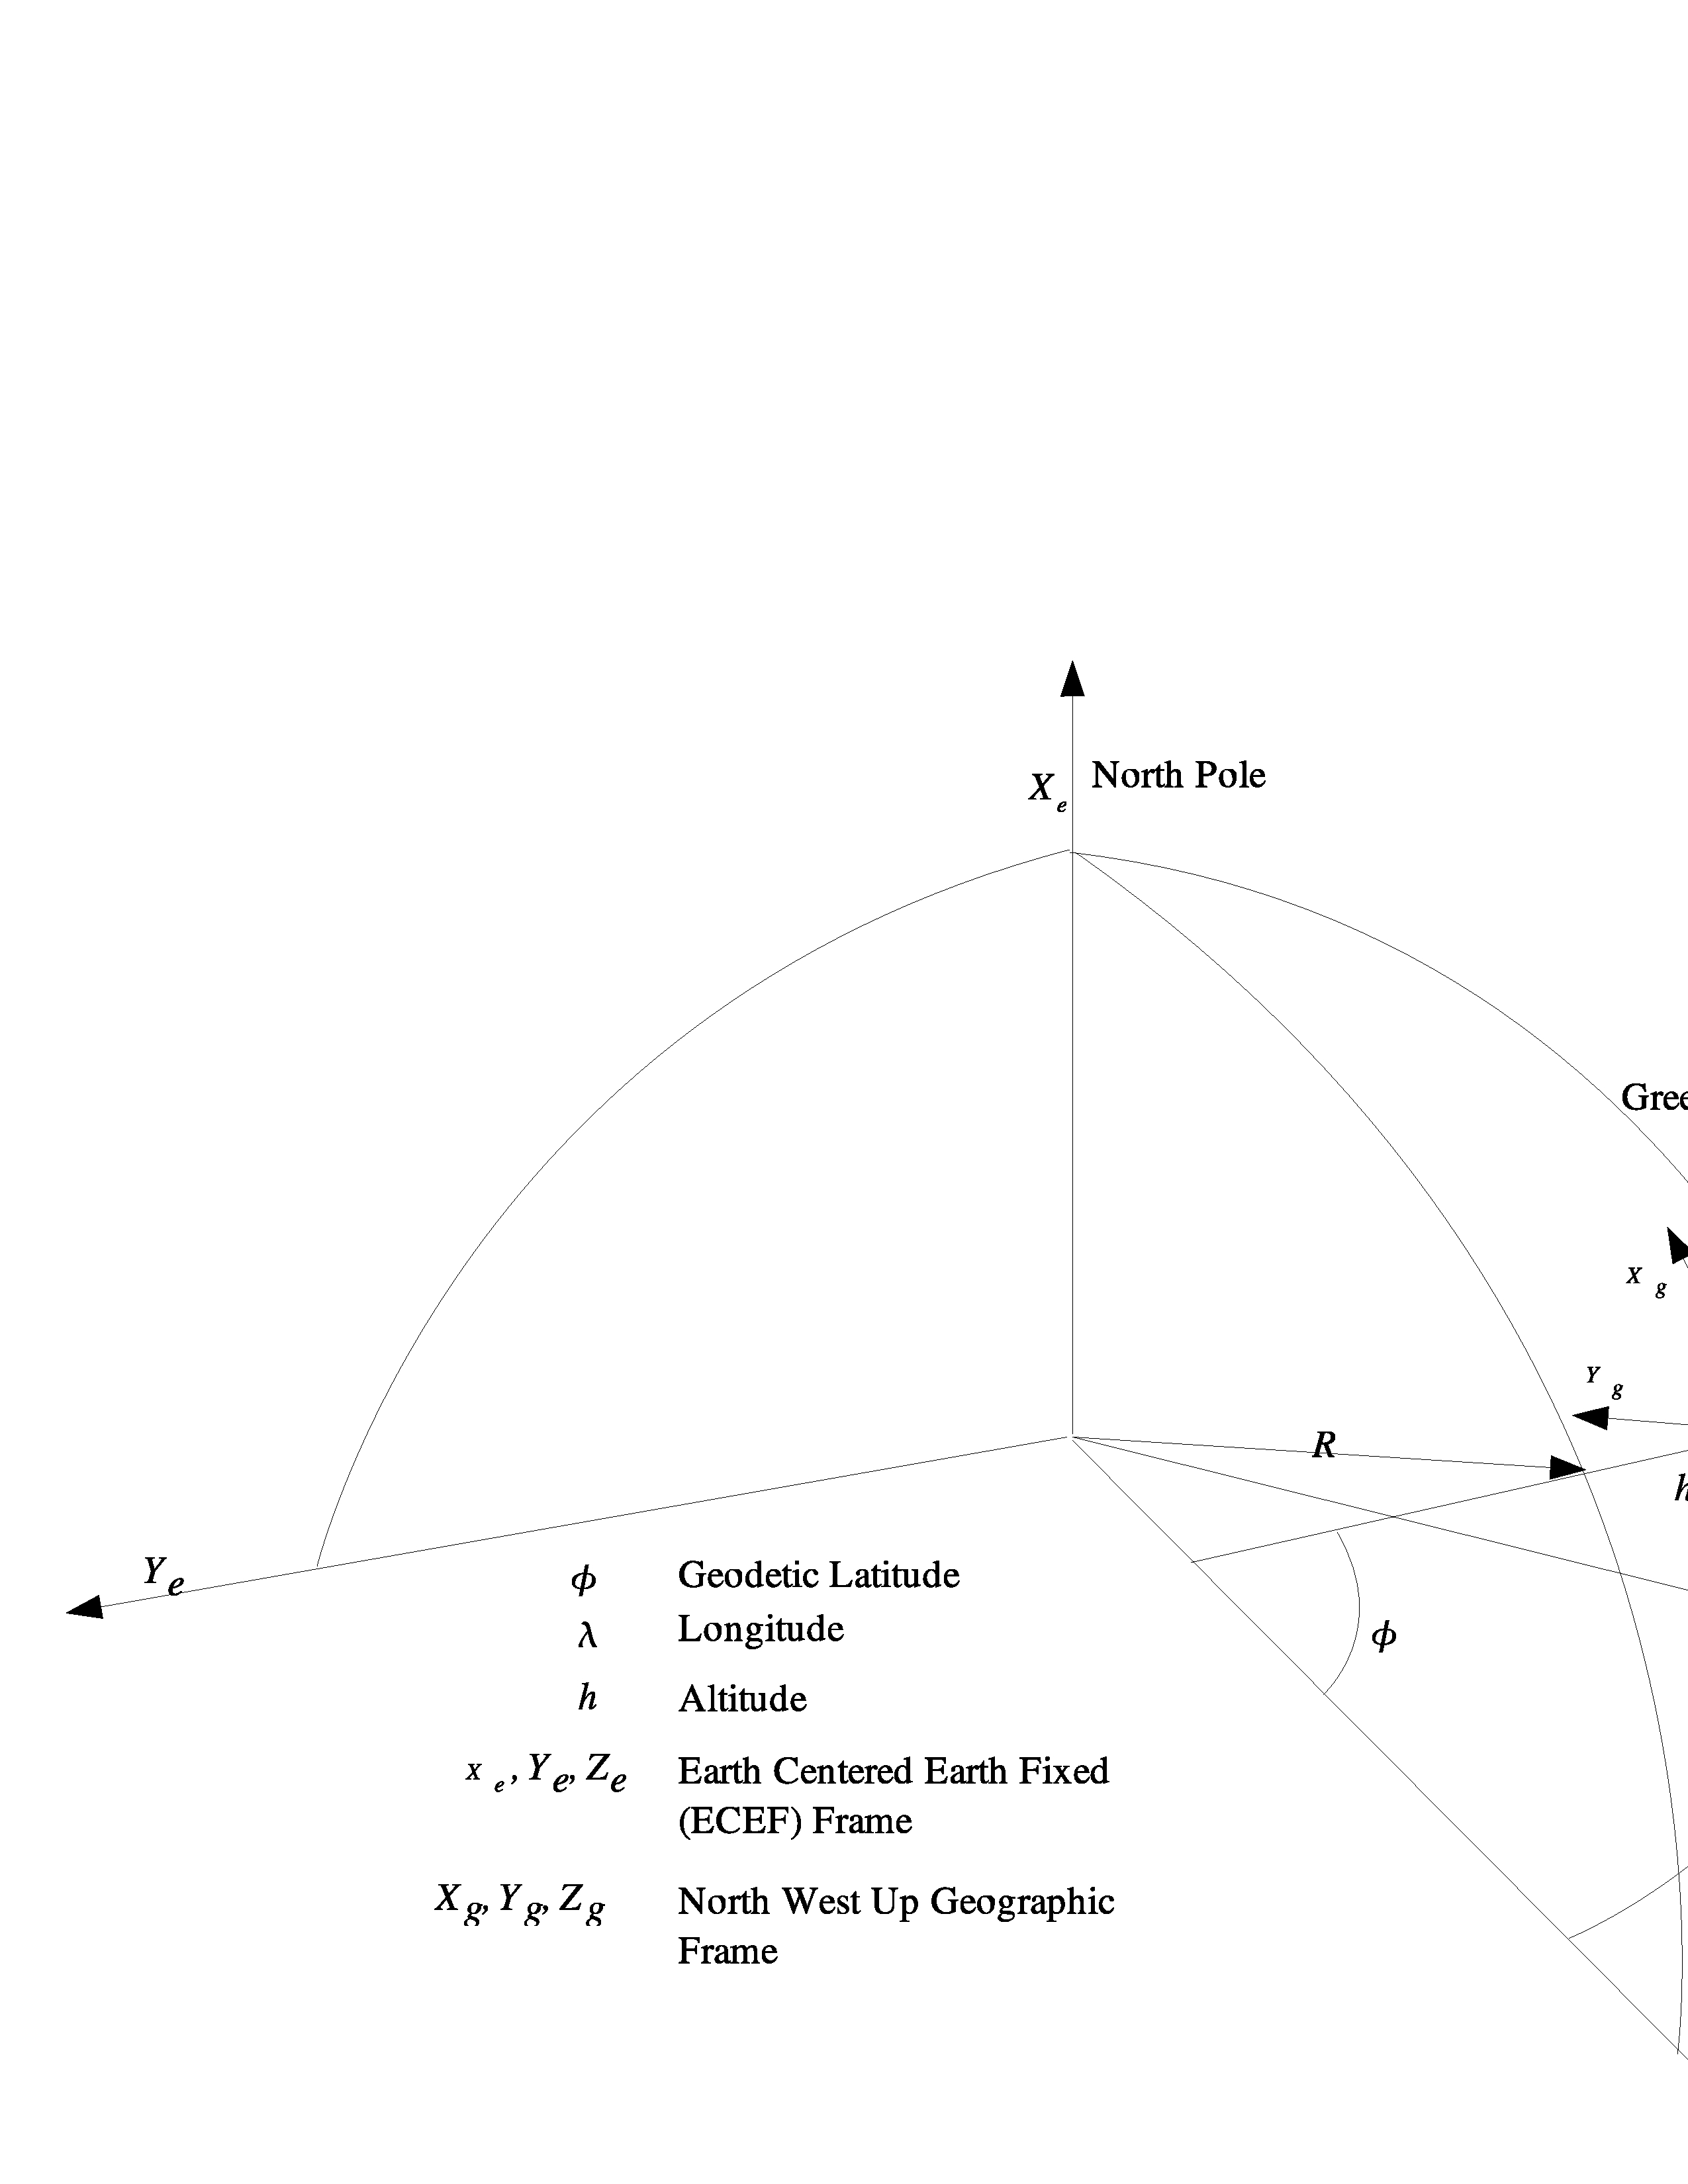
\includegraphics[width=\textwidth]{graphics/ecef.jpg}

\vfill
\end{frame}


\begin{frame}
Body Frame
 \begin{itemize}
 \item Attached to vehicle
 \item For aircraft:
   \begin{itemize}
    \item $X$ out the nose
    \item $Y$ out the right wing
    \item $Z$ down
   \end{itemize}
\end{itemize}
\end{frame}
\begin{frame}
Coordinate Frame Conversion
 \begin{itemize}
 \item All frames are earth-centered, hence differ only by
 rotation
 \item Rotation represented by direction cosine matrices (DCM)
 \begin{itemize}
	\item Represents the angles made by each of the basis vectors of one frame with those of the other
 \end{itemize}
 \item $\dcm{A}{B}$ = DCM transformation from frame A to frame B
\end{itemize}
\end{frame}
\begin{frame}
Coordinate Frame Conversion
\begin{itemize}
  \item "Direction Cosine" comes from dot product:
\[\ip{x}{y}=x\cdot y=\norm{x}\norm{y}\cos\theta_{xy}\]
where $\theta_{xy}$ is the angle between the two vectors $x$ and $y$.
  \item If $x$ and $y$ are unit vectors, then $\norm{x}=\norm{y}=1$ and we have:
\[\ip{x}{y}=x\cdot y=\cos\theta_{xy}\]
\end{itemize} 
\end{frame}

\begin{frame}
Coordinate Frame Conversion
\begin{itemize}
  \item If $U=\set{u_1,u_2,u_3}$ and $V=\set{v_1,v_2,v_3}$ are two sets of orthonormal basis vectors, then the DCM relating one frame to the other is given by:
\begin{align*}
\dcm{U}{V}&=
\begin{bmatrix}
\ip{u_1}{v_1} & \ip{u_1}{v_2} & \ip{u_1}{v_3}\\
\ip{u_2}{v_1} & \ip{u_2}{v_1} & \ip{u_2}{v_3}\\
\ip{u_3}{v_1} & \ip{u_3}{v_2} & \ip{u_3}{v_3}\\
\end{bmatrix}\\
&=
\begin{bmatrix}
\cos\theta_{11} & \cos\theta_{12} & \cos\theta_{13}\\
\cos\theta_{21} & \cos\theta_{22} & \cos\theta_{23}\\
\cos\theta_{31} & \cos\theta_{32} & \cos\theta_{33}\\
\end{bmatrix}
\end{align*}
\end{itemize} 
\end{frame}

\begin{frame}
Coordinate Frame Conversion
 \begin{itemize}
 \item DCMs are orthogonal matrices $\Rightarrow \left[\dcm{A}{B} \right]^{-1}=\left[\dcm{A}{B} \right]\trans$
 \item Third row (or column) is vector cross product of other two\\
 $\Rightarrow$ only six independent parameters
 \item DCMs satisfy:   $\dcm{B}{A}\dcm{C}{B}=\dcm{C}{A}$
\end{itemize}
\end{frame}
\begin{frame}
Coordinate Frame Conversion: Most important DCMs
 \begin{itemize}
 \item Body to Local Level: $\dcm{B}{L}$
 \begin{itemize}
 \item sometimes called Body to Nav and notated $\dcm{B}{N}$
 \item yields attitude info (Euler angles for roll, pitch, yaw)
 \end{itemize}
 \item Local Level to Earth: $\dcm{L}{E}$
 \begin{itemize}
 \item yields position info and also used to transform earth rate to
 local level
 \end{itemize}
\end{itemize}
\end{frame}
\begin{frame}
Coordinate Frame Conversion: Most important DCMs
\begin{itemize}
  \item Visualize $\dcm{L}{E}$'s determination of position as follows:
	\begin{itemize}
		\item As vehicle moves, local level frame changes its orienation with respect to earth's center in order to maintain local level with respect to earth's surface
		\item If you think of local level frame as attached to earth's surface, you get distracted by the displacement of the frame
		\item If you move local level frame to center of earth, the displacement disappears and all that remains are the rotations
	\end{itemize} 
\end{itemize} 
\end{frame}

\begin{frame}

%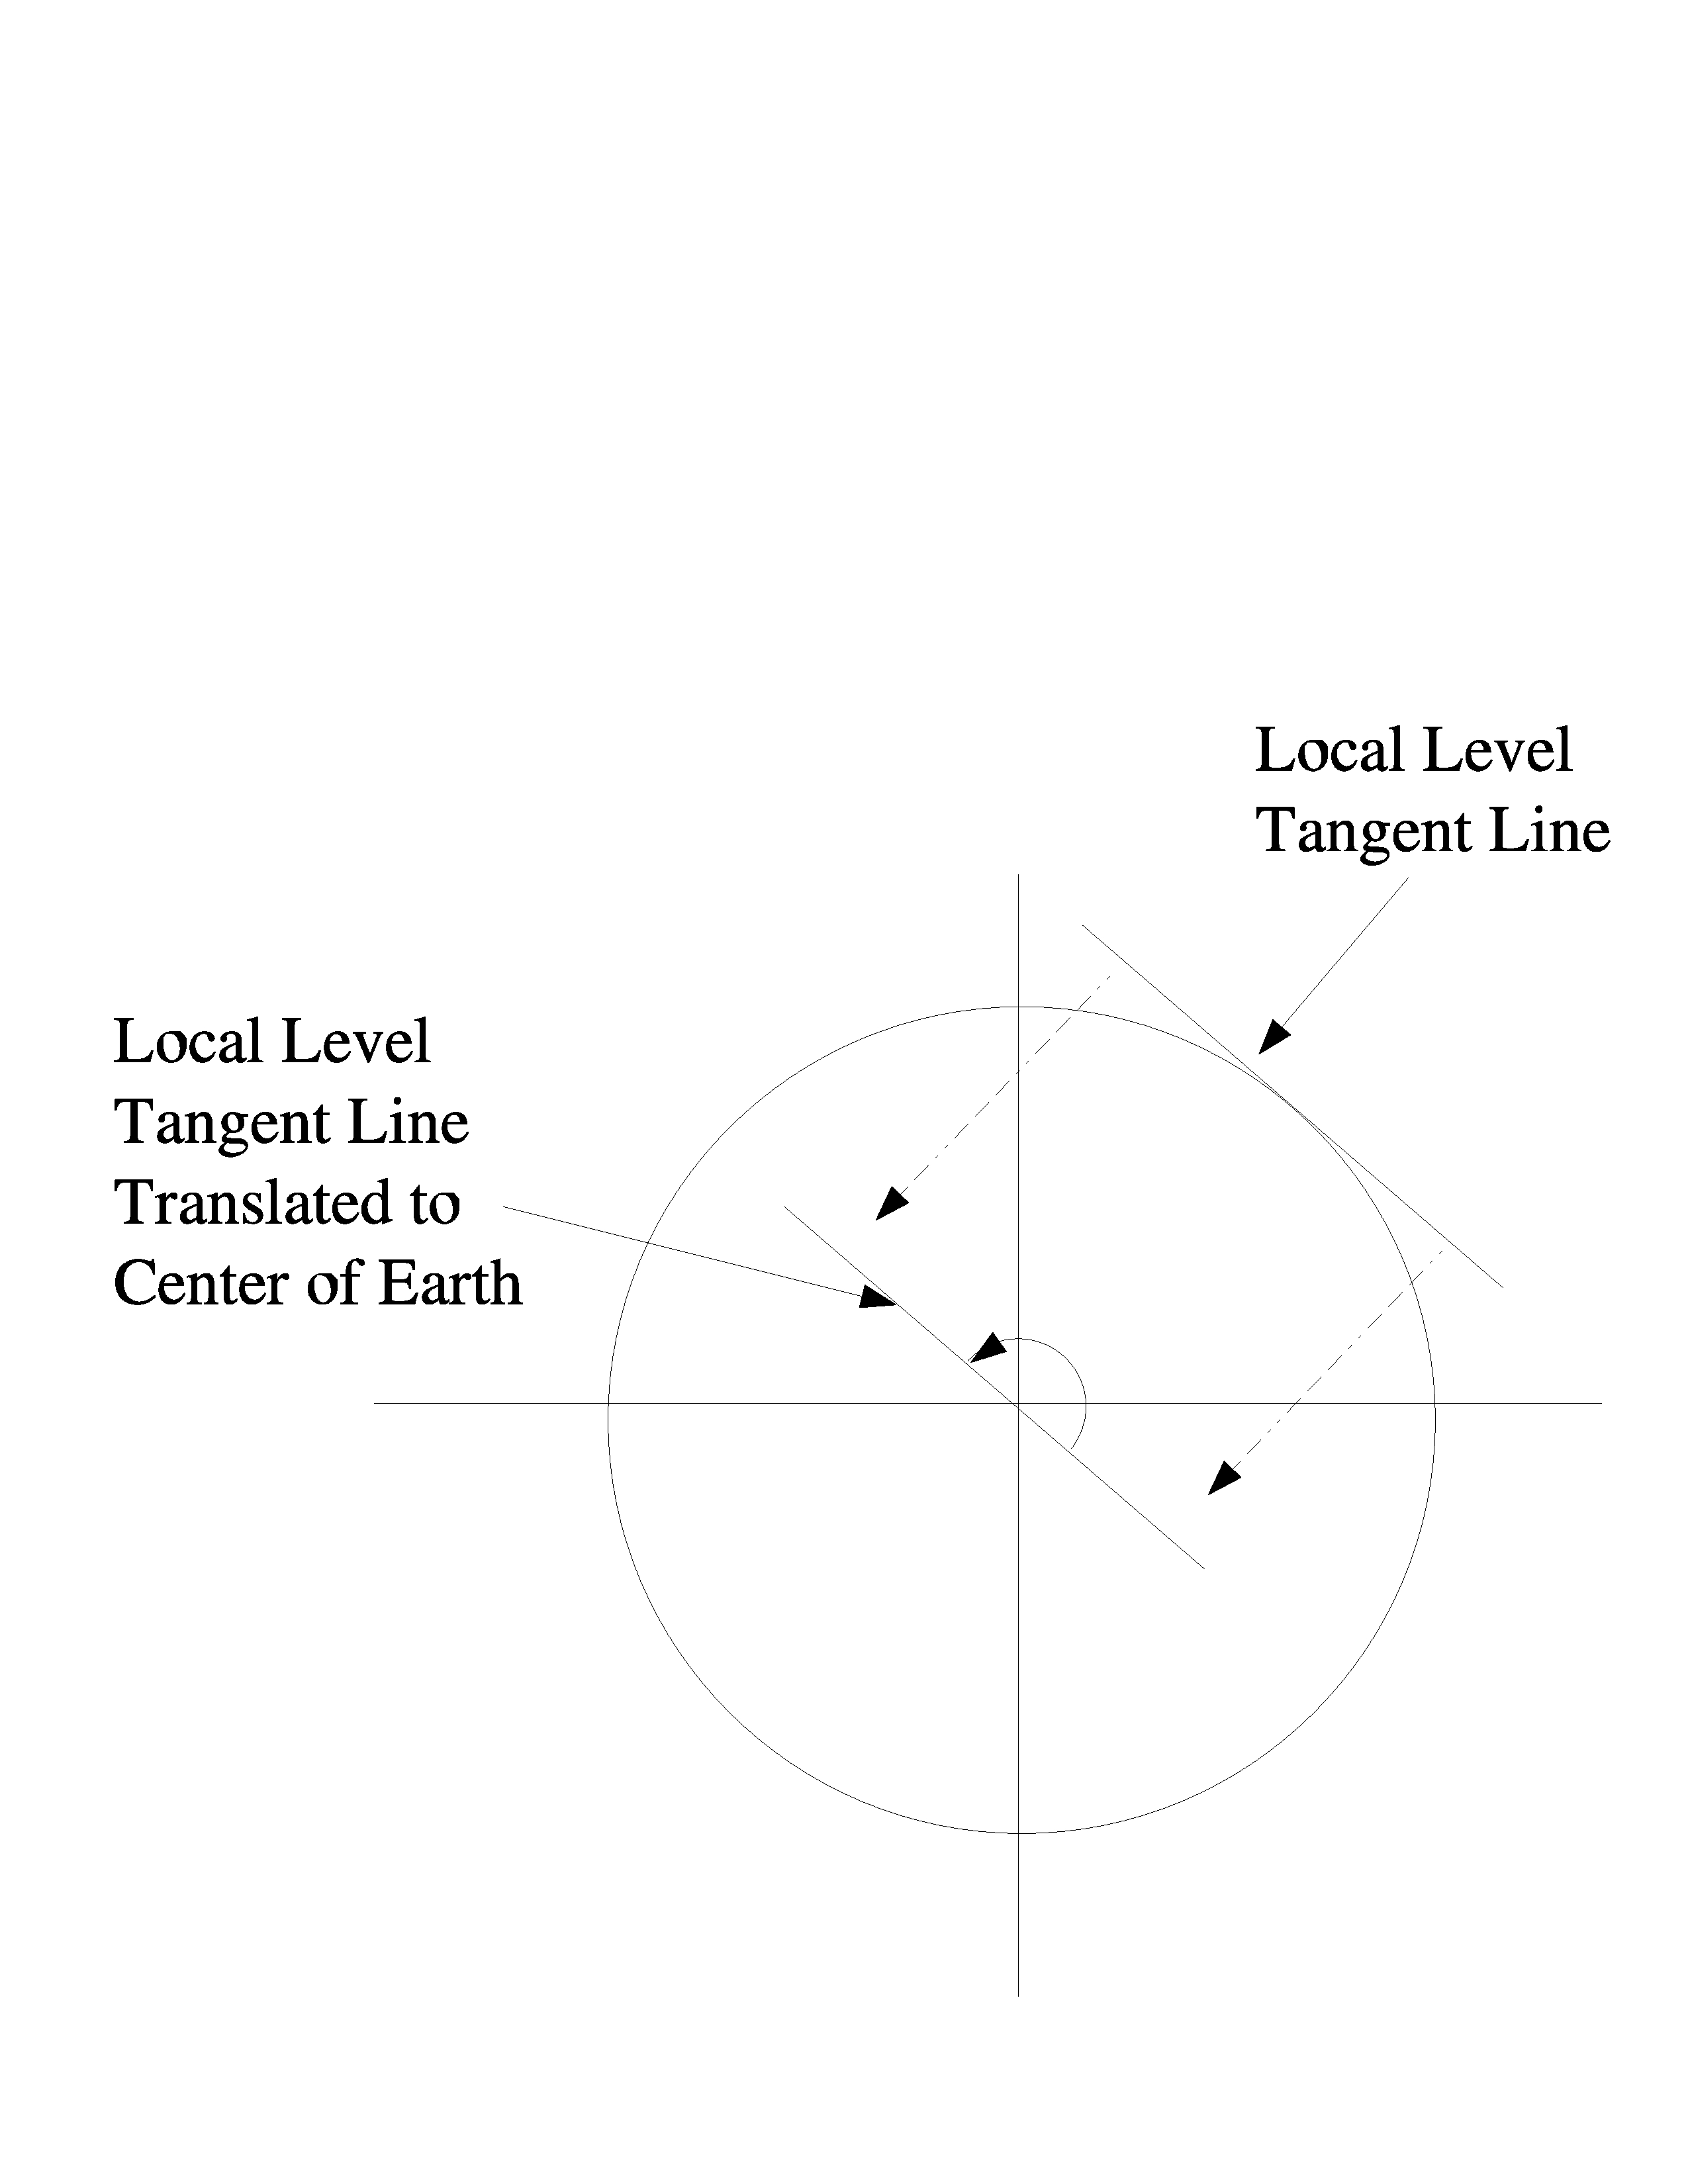
\includegraphics[width=\textwidth]{day3_seg2_navproblem/pos_dcm.jpg}

\end{frame}
% day3_seg1_navproblem/strapdown.tex
\begin{frame}
Strapdown Navigation:  Strapdown vs. Gimbaled
\begin{itemize}
  \item Gimbaled INS:
  \begin{itemize}
	\item Gyro stabilized platform
	\item Gimbal assembly and torque motors
	\item Resolvers, slip rings, bearings, etc. to control  platform
	\item Goal: Maintain stable, locally level or inertial reference frame
  \end{itemize}
\end{itemize} 
\end{frame}


\begin{frame}
Strapdown Navigation: Strapdown vs. Gimbaled
\begin{itemize}
  \item Gimbaled INS Issues
  \begin{itemize}
	\item Reliability and Cost: Lots of moving parts!
	\item Body rate and acceleration information not directly available
	\item Rate signals are generally noisy and have low bandwidth
  \end{itemize}
\end{itemize} 
\end{frame}


\begin{frame}
Strapdown Navigation: Strapdown vs. Gimbaled
\begin{itemize}
  \item Strapdown INS:
  \begin{itemize}
	\item Inertial instruments strapped to body frame
	\item Requires local level accelerations to be computed using direction cosine matrix $\dcm{B}{L}$
	\item $\dcm{B}{L}$ derived from gyro-sensed body rates
    \item Strapdown systems can be implemented with either rate gyros or attitude gyros 
  \end{itemize} 
\end{itemize} 
\end{frame}

\begin{frame}
Strapdown Navigation: Strapdown vs. Gimbaled
\begin{itemize}
  \item Strapdown INS Advantages
  \begin{itemize}
	\item Immediate detection of body rates and accelerations
	\item Fewer moving parts
	\item Potential redundancy advantages
  \end{itemize} 
  \item Gimbaled systems are nearly obsolete
\end{itemize} 
\end{frame}

\begin{frame}
%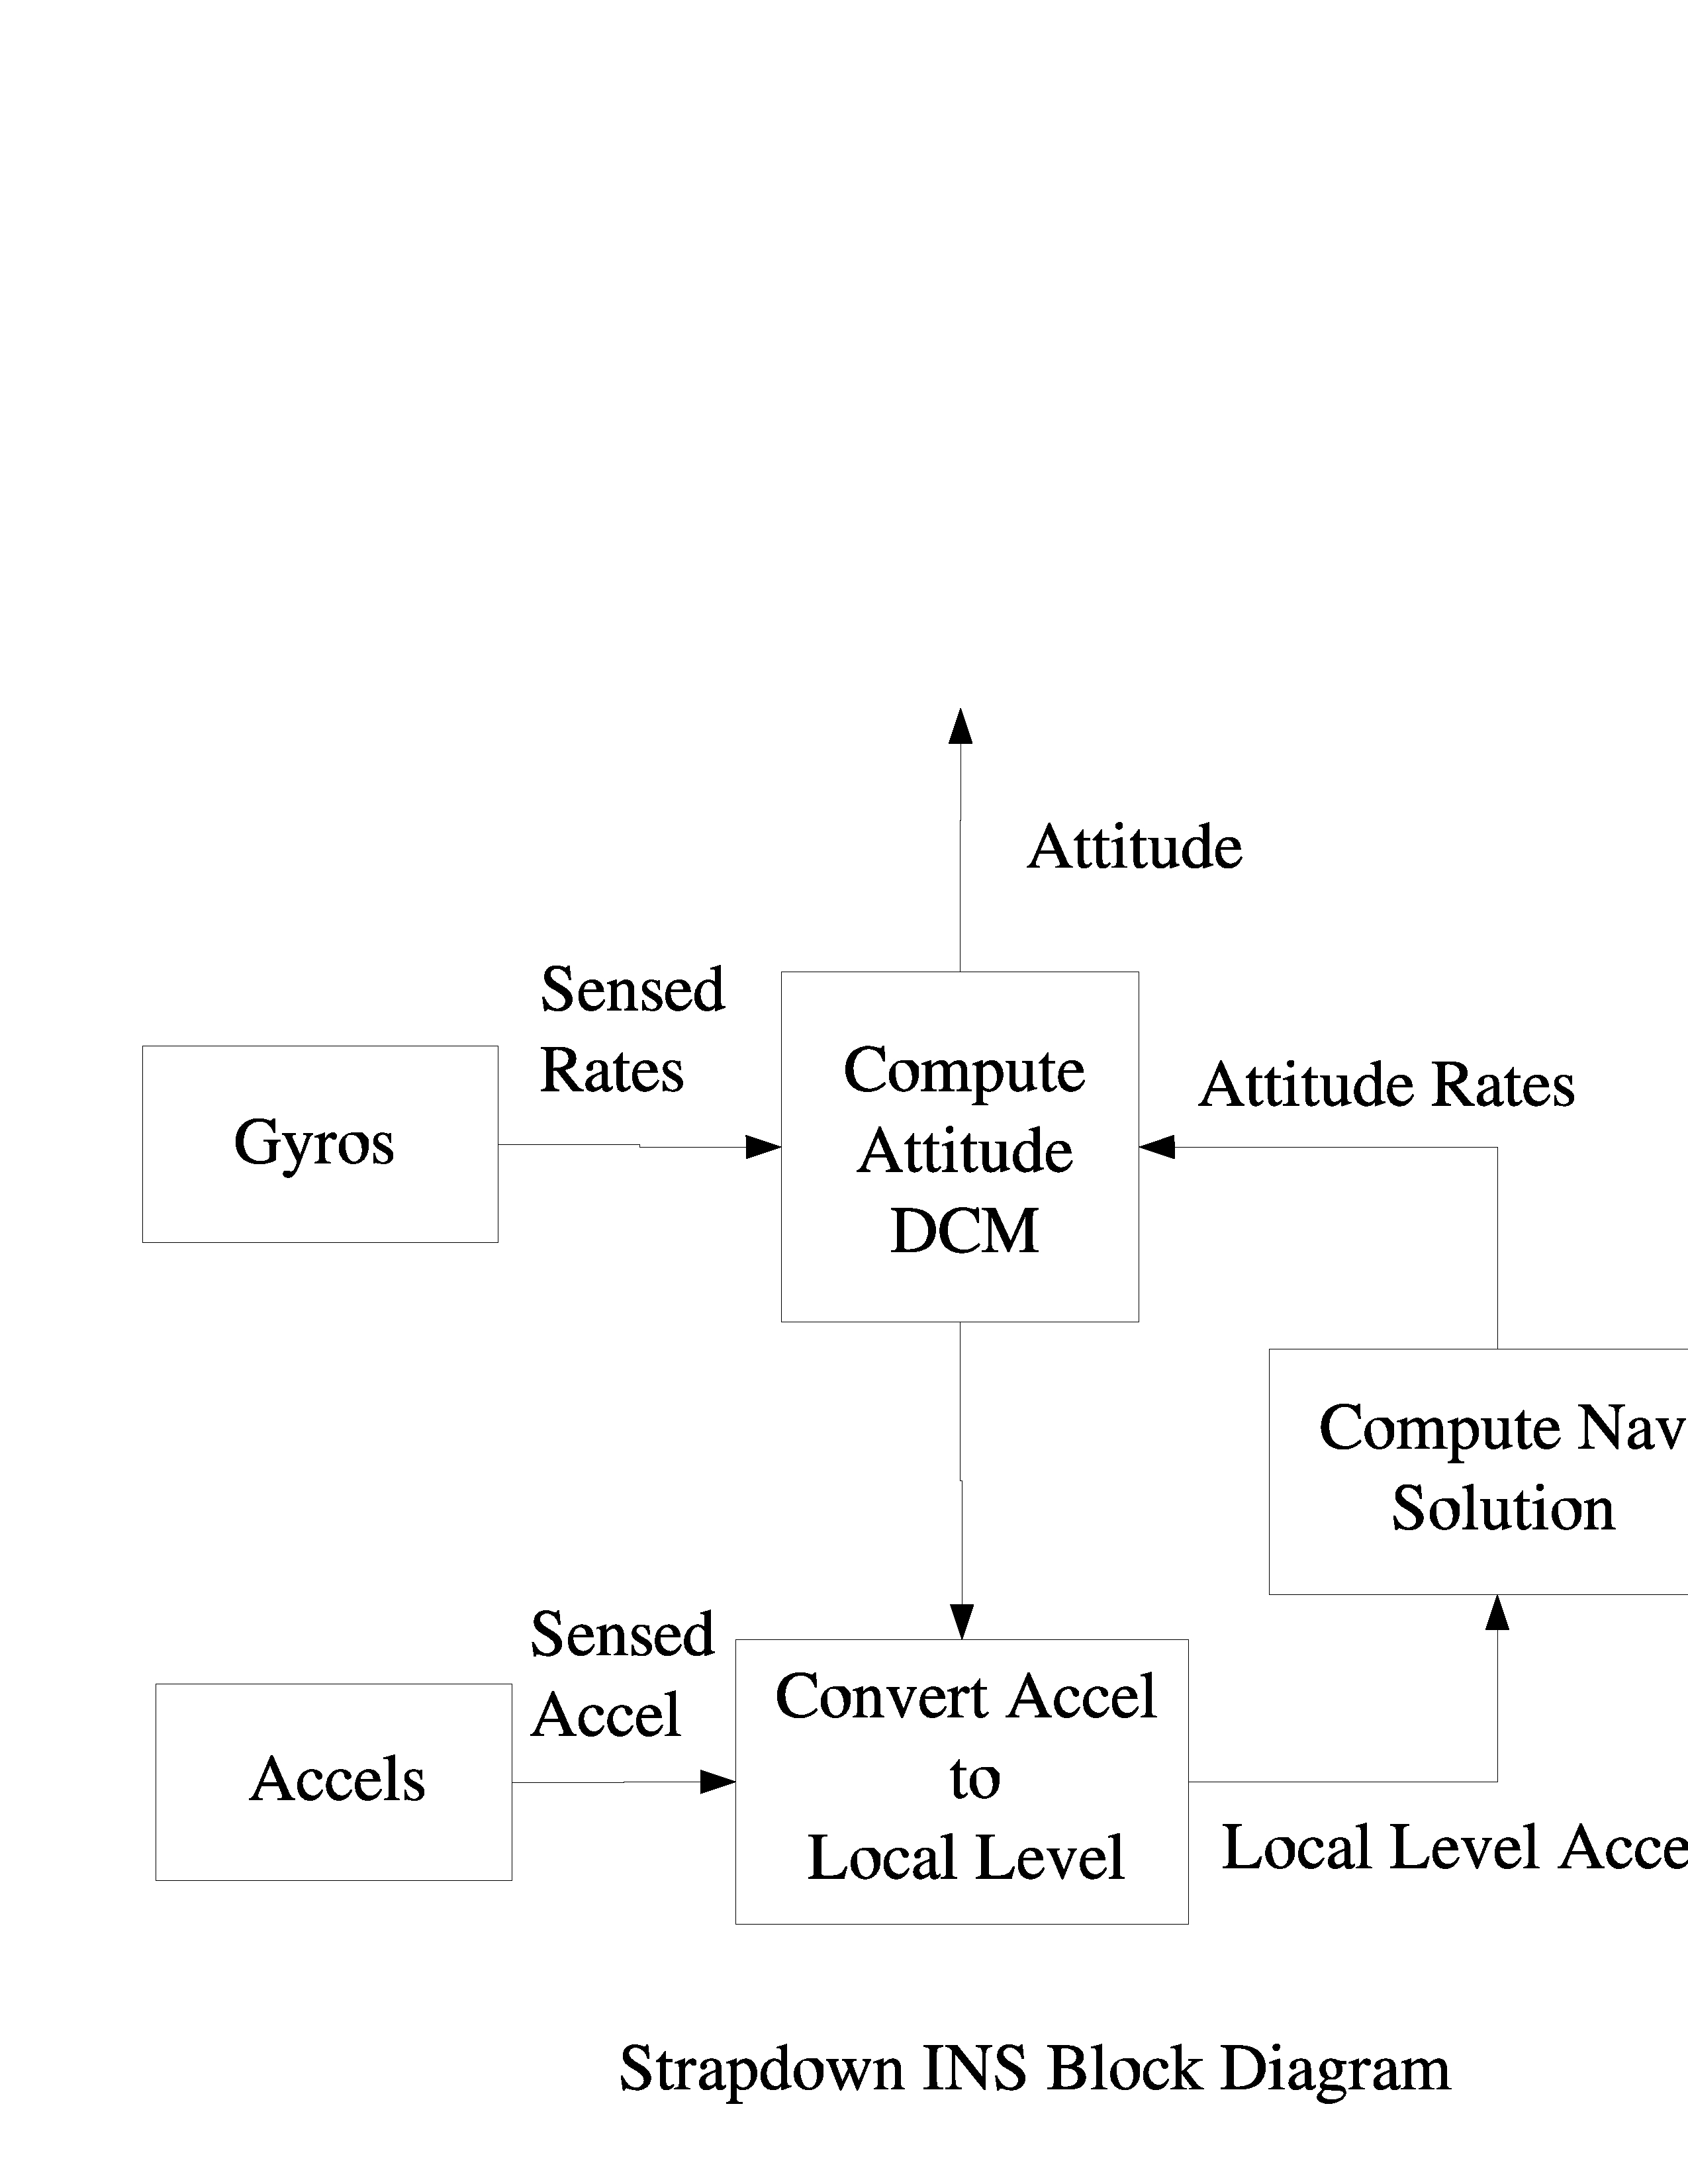
\includegraphics[width=\textwidth]{graphics/strapdown_block.jpg}
\end{frame}

\begin{frame}
Basic Strapdown Navigation Equations
 \begin{itemize}
 \item Need to compute attitude, velocity, and position
 \item I.e., need to compute $\dcm{B}{L}$ and $\dcm{L}{E}$
 \item These DCMs are dynamic quantities
 \item $\dcm{B}{L}$ determines attitude and can be rapidly varying
 \item $\dcm{L}{E}$ determines position and is slowly varying (relative to attitude dynamics)
\end{itemize}
\end{frame}

\begin{frame}
Rotating Coordinate Frames
\begin{itemize}
\item We first need to understand how an arbitrary vector and its time
derivatives in one coordinate frame are expressed in another frame
that is rotating with respect to the first.  
\item Let $A$ and $B$
denote two coordinate frames and assume that $B$ is rotating with
respect to $A$.  
\item We use the notation $\rotvec{A}{B}^A$ to express
the direction and magnitude of the rotation vector as seen in the $A$ frame.
\end{itemize}
\end{frame}
\begin{frame}
Rotating Coordinate Frames
\begin{itemize}
\item Every rotation vector can also be expressed as a skew symmetric
matrix.  
\item If $\omega$ is a rotation vector (without mentioning the
frames involved), then
\[\Omega = \skewsymmat{\omega}{1}{2}{3}.\]
\end{itemize}
\end{frame}
\begin{frame}
Rotating Coordinate Frames
\begin{itemize}
\item Since multiplication of a vector by the skew symmetric matrix
equivalent is the same thing as left multiplying the cross product
of the original vector, we can write:
\[\Omega v = \omega \times v\]
\item Therefore the notation $\xop{\omega}=\Omega$ is
common\footnote{One must be careful in making this identification
since left matrix multiplication is associative while left cross
product multiplication is not.}
\end{itemize}
\end{frame}

\begin{frame}
Rotating Coordinate Frames
\begin{itemize}
\item Let $v$ be an arbitrary vector in 3-space. 
\item Let
$\set{e_A^1,e_A^2,e_A^3}$ be orthonormal basis vectors in the $A$
frame 
\item Let $\set{e_B^1,e_B^2,e_B^3}$ be orthonormal basis
vectors in the $B$ frame\footnote{We reverse the roles of superscripts
and subscripts for basis vectors so that we may employ the
Einstein summation convention on occasion.}.  
\end{itemize}
\end{frame}

\begin{frame}
Rotating Coordinate Frames
\begin{itemize}
\item Thus, we can write
$v$ as $\sum_{i=1}^3 v_i^A e_A^i$ and also $\sum_{i=1}^3 v_i^B
e_B^i$. 
\item This is one and the same vector expressed in two different
coordinate frames\footnote{A vector is a linear combination of
basis vectors and not necessarily an ordered triple of real numbers.}.
\end{itemize}
\end{frame}
\begin{frame}
Rotating Coordinate Frames
\begin{itemize}
\item Note that, with respect to an arbitrary inertial
reference frame, we have for the time derivative:
\begin{align*}
  v &= \sum_{i=1}^3 v_i^A e_A^i = \sum_{i=1}^3 v_i^B e_B^i\\
    &\Rightarrow  \dot{v} = \dfrac{d}{dt}\left[ \sum_{i=1}^3 v_i^A e_A^i \right] = \dfrac{d}{dt}\left[\sum_{i=1}^3 v_i^B e_B^i
    \right]\\
    &\Rightarrow \sum_{i=1}^3 \left( \dot{v}_i^A e_A^i+ v_i^A
    \dot{e}_A^i\right)
    = \sum_{i=1}^3 \left(\dot{v}_i^B e_B^i+ v_i^B \dot{e}_B^i\right)\\
\end{align*}
\end{itemize}
\end{frame}
\begin{frame}
Rotating Coordinate Frames
\begin{itemize}
\item In the special case
that their respective coordinate frames are not rotating relative
to one another, each $\dot{e}_A^i = 0 = \dot{e}_B^i$.   
\item Nevertheless, regardless of rotation, we must always have:
\begin{equation}\label{scalarinveq}
  \scalarinveq.
\end{equation}
(Note that, in general, $\dot{v}_i^A\neq\dot{v}_i^B$.)
\end{itemize}
\end{frame}
\begin{frame}
Rotating Coordinate Frames
\begin{itemize}
\item Let frame $B$ rotate with respect to frame $A$ at a constant
rotational rate $\rotvec{A}{B}^A$ as expressed in $A$ frame coordinates.  
\item Since $B$ is not rotating with respect to itself, let us agree to label the quantity in Eq. \eqref{scalarinveq} as
$\dot{v}^B$. 
\item We'll assume that $A$ is an inertial frame and thus $\dot{v}=\dot{v}^A$.
\end{itemize}
\end{frame}
\begin{frame}
Rotating Coordinate Frames
\begin{itemize}
\item When viewed from the $A$ frame, however, it is not true that each
of the $\dot{e_i}^B$ is zero, since these unit vectors are slaved
to the $B$ frame and $B$ is rotating with respect to $A$ at rate
$\rotvec{A}{B}^A$.  
\item Therefore, we have:
\begin{equation}\label{aderiv}
\begin{split}
\dot{v}^A&=\sum_{i=1}^3 \dot{v}_i^A e_A^i + \sum_{i=1}^3 v_i^B
\dot{e}_B^i\\
         &=\sum_{i=1}^3 \dot{v}_i^B e_B^i + \sum_{i=1}^3 v_i^B
\dot{e}_B^i \text{\;\;\;\;(by Eq. \eqref{scalarinveq})}\\
         &=\dot{v}^B +\sum_{i=1}^3 v_i^B\dot{e}_B^i.
\end{split}
\end{equation}
\end{itemize}
\end{frame}

\begin{frame}
Rotating Coordinate Frames
\begin{itemize}
\item The last sum on the right side of Eq. \eqref{aderiv} can be
rewritten as the cross product $\rotvec{A}{B}^A\times v$, because
$\dot{e}_B^i=\rotvec{A}{B}^A\times e_B^i$, and
\begin{align*}
   \sum_{i=1}^3 v_i^B\dot{e}_B^i &= \sum_{i=1}^3 v_i^B\rotvec{A}{B}^A\times e_B^i \\
  &=\rotvec{A}{B}^A\times \sum_{i=1}^3 v_i^B e_B^i \\
  &=\rotvec{A}{B}^A\times v.
\end{align*}
\end{itemize}
\end{frame}
\begin{frame}
Rotating Coordinate Frames
\begin{itemize}
\item We thus arrive at the all-important Coriolis Equation which is
used often in navigation analysis:
\begin{equation}\label{corioliseq}
  \corioliseq.
\end{equation}
\end{itemize}
\end{frame}
\begin{frame}

Alternatively, we can express Eq. \eqref{corioliseq} in
skew-symmetric matrix form using
$\rotmat{A}{B}=\xop{\rotvec{A}{B}}$:
\begin{equation}\label{coriolismateq}
  \coriolismateq.
\end{equation}

Note that we must use superscripts on both $\rotmat{A}{B}$ and $v$
as soon as we make a commitment to a particular coordinate frame
representation.\footnote{Since matrices are defined in terms of
their action on basis vectors, it is appropriate to specify the
coordinate system.  On the other hand, if $\rotmat{A}{B}$ is taken
to be a linear transformation, then superscripts are not
necessary.}.

\end{frame}


\begin{frame}
Strapdown Navigation Equations
 \begin{itemize}
 \item Three differential equations
 \begin{itemize}
   \item Equation for body to local level transformation $\dcm{B}{L}$
   \item Equation for velocity (uses $\dcm{B}{L}$)
   \item Equation for local level to earth for position DCM $\dcm{L}{E}$
 \end{itemize}
\end{itemize}
\end{frame}
\begin{frame}
Strapdown Navigation Equations
 \begin{itemize}
 \item Two Algebraic Equations
 \begin{itemize}
   \item Equation for converting velocity to transport rate (to be explained)
   \item Equation for converting earth rate to local level
   coordinates
 \end{itemize}
\end{itemize}
\end{frame}
\begin{frame}
Strapdown Navigation Equations\\
The Three Differential Equations\\
\begin{equation}\label{cbleq}
  \cbleq
\end{equation}
\begin{equation}\label{strapveleq}
  \strapveleq
\end{equation}
\begin{equation}\label{cleeq}
  \cleeq
\end{equation}
\end{frame}
\begin{frame}
Strapdown Navigation Equations\\
The Two Algebraic Equations\\
\begin{equation}\label{trateeq}
  \trateeq \text{ (wander azimuth $\rho_z=0$)}
\end{equation}
\begin{equation}\label{erateeq}
  \erateeq
\end{equation}
\end{frame}
\begin{frame}
Strapdown Navigation Equations\\
The $\dcm{B}{L}$ Equation \eqref{cbleq}
\[\cbleq\]
\begin{itemize}
\item All the $\Omega$ matrices represent rotation vector cross products in skew-symmetric matrix format
\begin{itemize}
 \item $\rotmat{I}{B}^B$ is rotational rate of aircraft in body
coordinates
\item $\rotmat{I}{E}^L$ is earth rate in local level coordinates
\item $\rotmat{E}{L}^L$ is transport rate in local level
coordinates
\end{itemize}
\end{itemize}
\end{frame}
\begin{frame}
Strapdown Navigation Equations: Detour into Cross Product Matrices\\
\begin{itemize}
\item The cross product of $\omega=\colvecthree{\omega}{}$ with any other vector $v$ is the same as multiplying $v$ on the left by
$\Omega = \skewsymmat{\omega}{1}{2}{3}$
\item $\omega \times v=\Omega v$
\end{itemize}
\end{frame}
\begin{frame}
Strapdown Navigation Equations\\
The $\dcm{B}{L}$ Equation \eqref{cbleq}
\[\cbleq\]
\begin{itemize}
\item Transport rate is the rotational rate of the aircraft due to
motion over the surface of the earth.  Is a function of velocity.
\item $\rotmat{I}{B}^B$ is total inertial angular rate sensed by gyros and includes effects of
transport and earth rates.
\item Hence transport and earth rate effects have to be subtracted
off.
\end{itemize}
\end{frame}
\begin{frame}
Strapdown Navigation Equations\\
The Strapdown Velocity Equation \eqref{strapveleq}
\[\strapveleq\]
 \begin{itemize}
 \item Sometimes referred to as the velocity rate equation
 \item $\specforce^B$ is specific force sensed by accelerometers in
 body coordinates (because the accels are strapped to the body --
 hence the term strapdown)
\end{itemize}
\end{frame}
\begin{frame}
%\includegraphics[width=10in,height=6.5in]{strapnav_block.jpg}
\end{frame}
\begin{frame}
Strapdown Navigation Equations\\
The Transport Rate Equation \eqref{cleeq}
\[\cleeq\]
\begin{itemize}
  \item Connected to velocity rate equation by the first algebraic equation \eqref{trateeq}:
\[\trateeq\]
  \item Eq. \eqref{cleeq} Sometimes referred to as position rate equation, because $\dcm{L}{E}$ directly implies the vehicle position
\end{itemize} 
\end{frame}

\begin{frame}
Strapdown Navigation Equations\\
Position Rate / Transport Rate Equations (Geographic)
\begin{itemize}
  \item North transport rate:
\begin{equation}\label{trateneq}
\trateneq
\end{equation} 
  \item East transport rate:
\begin{equation}\label{trateeeq}
\trateeeq
\end{equation} 
where $e$ is ellipticity (approx. $\dfrac{1}{298}$) and $R_e$ is mean equatorial earth radius
\end{itemize} 
\end{frame}

\begin{frame}
Strapdown Navigation Equations\\
Position Rate / Transport Rate Equations (Geographic)
\begin{itemize}
  \item Latitude Rate:
\begin{equation}\label{latrate}
\latrateeq
\end{equation}  
  \item Longitude Rate:
\begin{equation}\label{lonrate}
\lonrateeq
\end{equation}  
\end{itemize} 
\end{frame}

\begin{frame}
Strapdown Navigation Equations\\
\begin{itemize}
  \item Geographic (north-slaved) mechanization has singularities at poles
  \item Two other approaches to local level coordinates:
  \begin{itemize}
	\item Free azimuth: vertical component of transport rate $\rho_z$= additive inverse of vertical component of earth rate
	\item Wander Azimuth:  vertical component of transport rate $\rho_z$ = 0
  \end{itemize}
\end{itemize} 
\end{frame}

\begin{frame}
Strapdown Navigation Equations\\
Position Rate / Transport Rate Equations (Wander and Free Azimuth)
\begin{itemize}
  \item X Transport Rate:
\begin{align}\label{xtrateeq}
\xtrateeq
\end{align}  
  \item Y Transport Rate:
\begin{align}\label{ytrateeq}
\ytrateeq
\end{align}  
\end{itemize} 
\end{frame}

\begin{frame}
Strapdown Navigation Equations\\
Position Rate / Transport Rate Equations (Wander and Free Azimuth)
\begin{itemize}
  \item Azimuth Rate:
\[
\rho_z= 
\begin{cases} 
-\erate d_{23}, &\text{if free azimuth;}\\ 
0,  &\text{if wander azimuth} 
\end{cases}
\]
  \item In equations above, the matrix $\left[d_{ij}\right]$ is the direction cosine matrix $\dcm{L}{E}$ from local level (L) frame to earth centered earth fixed (E) frame.
\end{itemize} 
\end{frame}

% day3_seg1_navproblem/exercises.tex
\begin{frame}
Exercises\\

1.  Compute direction cosine matrix $\dcm{U}{V}$, where 
\[U=\set{(1,0,0),(0,1,0),(0,0,1)}\] 
and \[V=\set{(-1,0,0),(0,1,0),(0,0,-1)}\]

2. Suppose you are starting at the equator and travelling due north, and your velocity is 5 m/sec.  Compute the transport rates $\rho_n$ and $\rho_e$ associated with this velocity and heading.  You may use the following constants: $\erateval$ and $\eradiusval$
\end{frame}


% day3_seg2_inertial/inertial_main.tex
\begin{frame}
  \onslide<1->{
	\frametitle{Inertial Error Dynamics} 
	\framesubtitle{Topics}
}
\begin{itemize}
  \onslide<2->{
 \item Imperfect Inertial Instruments
}
  \onslide<3->{
 \item From Strapdown Equations to Error Equations
}
  \onslide<4->{
 \item Initialization: Alignment
}
\end{itemize}
\end{frame}
% day3_seg2_inertial/impinst.tex
\begin{frame}
  \onslide<1->{
	\frametitle{Inertial Error Dynamics} 
	\framesubtitle{Imperfect Inertial Instruments}
}
\begin{itemize}
  \onslide<2->{
 \item Accelerometers and Gyros have inherent imperfections
}
  \onslide<3->{
 \item Bias, scale factor, $g^2$ terms, noise, random walks, etc.
}
  \onslide<4->{
 \item Inertial sensor clusters also have errors: misalignments
}
  \onslide<5->{
 \item Many error sources are calibrated out using rate tables during ATP
}
 \onslide<6->{ 
 \item Residual effects will influence strapdown nav equations
}
\end{itemize}
\end{frame}

\begin{frame}
  \onslide<1->{
	\frametitle{Inertial Error Dynamics} 
	\framesubtitle{Imperfect Inertial Instruments}
}
\begin{itemize}
  \onslide<2->{
  \item Strapdown nav equations very sensitive to gyro errors
}
  \onslide<3->{
  \item Gyro biases yield erroneous $\dcm{B}{L}$ matrix which in turn causes erroneous accelerations to be computed in local level frame
}
  \onslide<4->{
  \item Thus, gyro errors affect not only attitude, but also position and velocity
}
\end{itemize}
\end{frame}

\begin{frame}
  \onslide<1->{
	\frametitle{Inertial Error Dynamics} 
	\framesubtitle{Simple Inertial Error Models}
}
\begin{itemize}
  \onslide<2->{
  \item Gyros
\[
\simprateerreq{x}{y}{z}
\]
\[
\simprateerreq{y}{z}{x}
\]
\[
\simprateerreq{z}{x}{y}
\]

where $\gyrobias{i}$ is the $i^\text{th}$ gyro bias, $\gyrosf{i}$ the $i^\text{th}$ gyro scale factor, and $\gyromisalign{i}{j}$ is the misalignment of the $i^\text{th}$ gyro axis toward the $j^\text{th}$ gyro axis. 
}
\end{itemize}
\end{frame}

\begin{frame}
  \onslide<1->{
	\frametitle{Inertial Error Dynamics} 
	\framesubtitle{Simple Inertial Error Models}
}
\begin{itemize}
  \onslide<2->{
  \item Accelerometers
\[
\simpaccelerreq{x}{y}{z}
\]
\[
\simpaccelerreq{y}{z}{x}
\]
\[
\simpaccelerreq{z}{x}{y}
\]
where $\accelbias{i}$ is the $i^\text{th}$ accelerometer bias, $\accelsf{i}$ the $i^\text{th}$ accelerometer scale factor, and $\accelmisalign{i}{j}$ is the misalignment of the $i^\text{th}$ accelerometer axis toward the $j^\text{th}$ accelerometer axis. 
}
\end{itemize}
\end{frame}


\begin{frame}
  \onslide<1->{
	\frametitle{Inertial Error Dynamics} 
	\framesubtitle{Bias Models}
}
\begin{itemize}
  \onslide<2->{
  \item Bias in both types of instruments can be further broken down into several components:
  \begin{itemize}
	\item fixed bias -- constant from turn-on to turn-on -- should be calibrated out
	\item bias stability -- varies from turn-on to turn-on -- can't be calibrated out, but can be characterized in terms of variance -- can model as random constant
	\item bias drift -- usually modeled as random walk
  \end{itemize} 
}
\end{itemize}
\end{frame}


\begin{frame}
  \onslide<1->{
	\frametitle{Inertial Error Dynamics} 
	\framesubtitle{Scale Factor Models}
}
\begin{itemize}
  \onslide<2->{
  \item Scale factor can also be modeled as a sum of three components
}
  \onslide<3->{
  \item Often in nav filters, scale factor residual is modeled as a random constant
}
  \onslide<4->{
  \item Important to keep in mind that the contribution of scale factor error is a function of input (rate or acceleration) 
}
\end{itemize}
\end{frame}
\begin{frame}
  \onslide<1->{
	\frametitle{Inertial Error Dynamics} 
	\framesubtitle{Higher Order Models}
}
\begin{itemize}
  \onslide<2->{
  \item In expanding the output error as a Taylor series function of input, bias, scale factor, and misalignment show up as zero and first order terms.
}
  \onslide<3->{
  \item Higher order terms are also present, especially second order terms.
}
  \onslide<4->{
  \item In some calibration and alignment filters, such higher order effects are modelled
}
  \onslide<5->{
  \item SNU-84-1 includes error budgets associated with all the combined, higher order effects.  
}
\end{itemize}
\end{frame}

\begin{frame}
  \onslide<1->{
	\frametitle{Inertial Error Dynamics} 
	\framesubtitle{Higher Order Models:  Taylor Series of Two Variables}
}
  \onslide<2->{
\begin{align*}
\gentaylordouble{f}{x}{y}{x_0}{y_0}
\end{align*}
Taylor Series provides basis for all error analysis.
}
\end{frame}

\subsection{Strapdown Error Dynamics}
% day3_seg2_inertial/straperr.tex
\begin{frame}
  \onslide<1->{
	\frametitle{Inertial Error Dynamics} 
	\framesubtitle{From Strapdown Equations to Error Equations}
}
\begin{itemize}
  \onslide<2->{
 \item Nav equations require perfect inertial instruments
}
  \onslide<3->{
 \item Instruments are not perfect
}
  \onslide<4->{
 \item Inertial instrument error sources (bias, scale factor errors, etc.) generate erroneous rate and acceleration inputs to the nav equations  
}
  \onslide<5->{
 \item Need to figure out the effects on the outputs of these equations
}
\end{itemize}
\end{frame}
% cm_kf_talk_straperr.tex


\begin{frame}
  \onslide<1->{
	\frametitle{Inertial Error Dynamics} 
	\framesubtitle{Strapdown Error Equations}
}
\begin{itemize}
  \onslide<2->{
 \item Nature of Errors
}
  \onslide<3->{
 \item Error Operator
}
  \onslide<4->{
 \item Error Equations
}
\end{itemize}
\end{frame}


\begin{frame}
  \onslide<1->{
	\frametitle{Inertial Error Dynamics} 
	\framesubtitle{Strapdown Error Equations: Nature of Errors}
}
\begin{itemize}
  \onslide<2->{
 \item Errors propagate according to derived equations
}
  \onslide<3->{
 \item Errors are generally small, so approximating assumptions
 help simplify the math
 \begin{itemize}
}
  \onslide<4->{
 \item linearize otherwise non-linear dynamics
}
  \onslide<5->{
 \item small angle assumptions:  $\sin\theta \approx \theta$
 \end{itemize}
}
\end{itemize}
\end{frame}


\begin{frame}
  \onslide<1->{
	\frametitle{Inertial Error Dynamics} 
	\framesubtitle{Strapdown Error Equations: Error Operator}
}
\begin{itemize}
  \onslide<2->{
\item   If $A$ is any quantity, we define error operator as follows:
\begin{equation}\label{errop}
  \errop{A},
\end{equation}
where $A$ is the true quantity of interest and $\hat{A}$ is an
apparent quantity.  The latter could be a measured value, and
estimated value, or some computed value.  This means that
\[\hat{A}=A+\delta A\]
i.e., the apparent value is the true value plus some error.

}
\end{itemize}
\end{frame}


\begin{frame}
  \onslide<1->{
	\frametitle{Inertial Error Dynamics} 
	\framesubtitle{Strapdown Error Equations: Error Operator}
}
\begin{itemize}
  \onslide<2->{
\item   Error operator satisfies:
\begin{equation}\label{erropid}
  \delta(AB) = \delta A \cdot B + A \cdot \delta B
\end{equation}
}
  \onslide<3->{
\item   Proof:
\begin{align*}
\delta(AB) &= \widehat{AB} - AB\\
&= \hat{A}\hat{B}-AB\\
&= (A+\delta A)(B+\delta B)-AB\\
&= AB + A\cdot\delta B +\delta A \cdot B + \delta A \cdot \delta B - AB\\
& = \delta A \cdot B + A\cdot\delta B
\end{align*}
since we may assume that $\delta A \cdot\delta B \approx 0$.
}
\end{itemize}
\end{frame}


\begin{frame}
  \onslide<1->{
	\frametitle{Inertial Error Dynamics} 
	\framesubtitle{Strapdown Error Equations}
}
\begin{itemize}
  \onslide<2->{
\item   Applying these to the three differential equations, yields three
error equations:
\begin{equation}\label{cblerreq}
  \cblerreq
\end{equation}
\begin{equation}\label{strapvelerreq}
  \strapvelerreq
\end{equation}
\begin{equation}\label{cleerreq}
  \cleerreq
\end{equation}
}
\end{itemize}
\end{frame}



\begin{frame}
  \onslide<1->{
	\frametitle{Inertial Error Dynamics} 
	\framesubtitle{Strapdown Error Equations}
}
\begin{itemize}
  \onslide<2->{
\item   Introducing \textbf{small angular rotations} for tilt and position
\begin{itemize}
}
  \onslide<3->{
  \item $\compdcm{B}{L}$, the computed (i.e., apparent) version of $\dcm{B}{L}$ is related additively to the true version by the error $\delta \dcm{B}{L}$
\[\compdcm{B}{L}= \dcm{B}{L}+ \delta \dcm{B}{L}\]
}
  \onslide<4->{
  \item It is also related to $\dcm{B}{L}$ by a small direction cosine matrix relating the local level frame to the computer frame $\widehat{L}$:
\[\compdcm{B}{L}= \dcm{L}{\widehat{L}}\dcm{B}{L}\] 
\end{itemize} 
}
\end{itemize}
\end{frame}

\begin{frame}
  \onslide<1->{
	\frametitle{Inertial Error Dynamics} 
	\framesubtitle{Strapdown Error Equations}
}
\begin{itemize}
  \onslide<2->{
\item Substituting the second equation into the first allows us to solve for $\delta \dcm{B}{L}$:
\begin{align*}
\delta \dcm{B}{L} &= \compdcm{B}{L} -\dcm{B}{L}\\
&= \dcm{L}{\widehat{L}}\dcm{B}{L}-\dcm{B}{L}\\
&= (\dcm{L}{\widehat{L}} - I)\dcm{B}{L}
\end{align*}
Now, let's introduce $\Phi=I-\dcm{L}{\widehat{L}}$ to obtain:
\[\delta \dcm{B}{L}=-\Phi\dcm{B}{L}\]
}
\end{itemize}
\end{frame}


\begin{frame}
  \onslide<1->{
	\frametitle{Inertial Error Dynamics} 
	\framesubtitle{Strapdown Error Equations}
}
\begin{itemize}
  \onslide<2->{
  \item Using small angle approximations, $\dcm{L}{\widehat{L}}$ can be written in the form
\[\dcm{L}{\widehat{L}}=
\begin{bmatrix}
1&\phi_z&-\phi_y\\
-\phi_z&1&\phi_x\\
\phi_y&-\phi_x&1
\end{bmatrix}.
\]
Thus, $\Phi=I-\dcm{L}{\widehat{L}}$ is seen to be a skew-symmetric rotation matrix:
\[\Phi=
\begin{bmatrix}
0&-\phi_z&\phi_y\\
\phi_z&0&-\phi_x\\
-\phi_y&\phi_x&0
\end{bmatrix}.
\]
}
\end{itemize}
\end{frame}


\begin{frame}
  \onslide<1->{
	\frametitle{Inertial Error Dynamics} 
	\framesubtitle{Strapdown Error Equations}
}
\begin{itemize}
  \onslide<2->{
  \item $\Phi$ is therefore equal to the cross product operator associated with a vector $\phi^L = \begin{bmatrix}\tiltx^L & \tilty^L & \az^L \end{bmatrix}\trans$.  I.e.,
\[\Phi = \xop{\phi^L}\]
}
  \onslide<3->{
\item The three components of $\phi^L$ will become three states in our inertial error dynamics Kalman filter.
}
  \onslide<4->{
\item $\phi_x$ and $\phi_y$ are called tilts, while $\psi_z$ is called the azimuth error.
}
\end{itemize}
\end{frame}


\begin{frame}
  \onslide<1->{
	\frametitle{Inertial Error Dynamics} 
	\framesubtitle{Strapdown Error Equations}
}
\begin{itemize}
  \onslide<2->{
  \item By a similar derivation, we can introduce a small angular position angle error $e^L=\begin{bmatrix}e_x^L & e_y^L & e_z^L \end{bmatrix}\trans$
}
  \onslide<3->{
  \item $e^L$ is associated with $\delta\dcm{E}{L}$ just as $\phi^L$ is associated with $\delta\dcm{B}{L}$:
\[\delta\dcm{E}{L}=-E^L\dcm{E}{L},\]
where $E^L$ is the skew-symmetric matrix form of $e^L$.
}
  \onslide<4->{
  \item The three components of $e^L$ yield the three position error states in a typical navigation Kalman filter.
}
\end{itemize}
\end{frame}


\begin{frame}
  \onslide<1->{
	\frametitle{Inertial Error Dynamics} 
	\framesubtitle{Strapdown Error Equations}
}
\begin{itemize}
  \onslide<2->{
  \item We are working to simplify Eq. \eqref{cblerreq}:
\[\cblerreq\]
}
  \onslide<3->{
  \item We have an expression for $\delta \dcm{B}{L}$.
}
\end{itemize}
\end{frame}


\begin{frame}
  \onslide<1->{
	\frametitle{Inertial Error Dynamics} 
	\framesubtitle{Strapdown Error Equations}
}
\begin{itemize}
  \onslide<2->{
  \item Consider the earth rate error term $\delta \rotmat{I}{E}^L$.  Since $\rotmat{I}{E}^L=\dcm{E}{L}\rotmat{I}{E}^E$ and $\delta\rotmat{I}{E}^E=0$, we derive:
\[\delta\rotmat{I}{E}^L=\delta\dcm{E}{L}\rotmat{I}{E}^E.\]
}
  \onslide<3->{
  \item But $\delta\dcm{E}{L}=-E^L\dcm{E}{L}$.  Therefore,
\begin{align*}
\delta\rotmat{I}{E}^L&=-E^L\dcm{E}{L}\rotmat{I}{E}^E\\
&=-E^L\rotmat{I}{E}^L.
\end{align*}
}
\end{itemize}
\end{frame}


\begin{frame}
  \onslide<1->{
	\frametitle{Inertial Error Dynamics} 
	\framesubtitle{Strapdown Error Equations}
}
\begin{itemize}
  \onslide<2->{
  \item For the error in transport rate, $\delta\rotmat{E}{L}^L$, using the error operator on Eq. \eqref{trateeq}, a new error terms having to do with altitude error shows up:
\begin{align*}
\delta\rotvec{E}{L}^L&=\delta\left[\dfrac{1}{R}u_r^L\times v^L\right]\\
&=\dfrac{1}{R}u_r^L\times \delta v^L - \dfrac{\delta h}{R^2}\left[u_r^L\times v^L\right]
\end{align*}
}
  \onslide<3->{
\item Here, $R=R_e+h$ for a spherical earth of radius $R_e$.
}
\end{itemize}
\end{frame}


\begin{frame}
  \onslide<1->{
	\frametitle{Inertial Error Dynamics} 
	\framesubtitle{}
}
\begin{itemize}
  \onslide<2->{
  \item Eq. \eqref{cblerreq} can now be rewritten as:
\begin{equation}\label{tilteq}
\tilteq
\end{equation} 
where $\delta \rotmat{E}{L}^L$ is the skew-symmetric matrix form of 
\[\trateerreqsphere\]
}
\end{itemize}
\end{frame}


\begin{frame}
  \onslide<1->{
	\frametitle{Inertial Error Dynamics} 
	\framesubtitle{Strapdown Error Equations}
}
\begin{itemize}
  \onslide<2->{
  \item Similarly, the velocity equation can be rewritten:
\begin{align*}
\velerreq
\end{align*} 
while the equation for the position angle error $e^L$ itself is
\begin{equation}
\paeeq
\end{equation} 
}
\end{itemize}
\end{frame}




\begin{frame}
  \onslide<1->{
	\frametitle{Inertial Error Dynamics} 
	\framesubtitle{Strapdown Error Equations}
}
\begin{itemize}
  \onslide<2->{
\item   Further Simplifications Using Telescope Pointing Angle Error

}
  \onslide<3->{
  \item $\psi^L = \phi^L - e^L$
}
  \onslide<4->{
  \item Leads to:
}
  \onslide<5->{
\begin{equation}\label{deltardoteq}
\deltardoteq
\end{equation}
and
\begin{eqnarray}
\velerreqpsi
\end{eqnarray}  
}
\end{itemize}
\end{frame}



\begin{frame}
  \onslide<1->{
	\frametitle{Inertial Error Dynamics} 
	\framesubtitle{Strapdown Error Equations}
}
\begin{itemize}
  \onslide<2->{
  \item Finally, the equations for the telescope pointing angle errors are: 
}
  \onslide<3->{
\begin{equation}\label{telscopeeq}
\telscopeeq
\end{equation}
}
\end{itemize}
\end{frame}

\begin{frame}
  \onslide<1->{
	\frametitle{Inertial Error Dynamics} 
	\framesubtitle{Strapdown Error Equations}
}
\begin{itemize}
  \onslide<2->{
 \item Three error equations yield three vector quantities of
 interest
 \begin{itemize}
}
  \onslide<3->{
 \item position error vector (3) $\poserr$ derived from $\delta \dcm{L}{E}$
}
  \onslide<4->{
 \item velocity error vector (3) $\velerr^L$ (or $\delta v^L$)
}
  \onslide<5->{
 \item attitude error vector (3) $\tiltx,\tilty,\az$ from $\delta \dcm{B}{L}$
 \end{itemize}
}
\end{itemize}
\end{frame}

\begin{frame}
  \onslide<1->{
	\frametitle{Inertial Error Dynamics} 
	\framesubtitle{Strapdown Error Equations}
}
\begin{itemize}
  \onslide<2->{
  \item See Matlab / Simulink Models
	\begin{itemize}
}
  \onslide<3->{
	  \item Strapdown Navigation Equations: TBD
}
  \onslide<4->{
	  \item Strapdown Navigation Error Equations: TBD
    \end{itemize}
}
\end{itemize}
\end{frame}


\subsection{Inertial Alignment}
% day3_seg2_inertial/align.tex
\begin{frame}
Initialization:  Alignment
 \begin{itemize}
 \item Coarse Leveling
  \begin{itemize}
    \item Gimbal system limited by platform torquing rates
    \item Strapdown systems have no real rate limits
    \item Time average of accel outputs scaled by $1/g$
	\item Yields third row of DCM to begin fine alignment
  \end{itemize}
 \item Fine Alignment
 \item Alignment filter aids in further leveling
\end{itemize}
\end{frame}

%% day3_seg2_inertial/exercises.tex
\begin{frame}
Exercises
 \begin{itemize}
 \item
 \item
 \item
\end{itemize}
\end{frame}


% day3_seg3_9-state/9-state_main.tex
\begin{frame}
  \onslide<1->{
	\frametitle{The Basic 9-State Kalman Filter} 
	\framesubtitle{Topics}
}
\begin{itemize}
  \onslide<2->{
 \item Whole State Filters vs. Error State Filters
}
  \onslide<3->{
 \item The Canonical Nine States
}
  \onslide<4->{
 \item INS Error State Dynamics and Transition Matrix
}
\end{itemize}
\end{frame}
% day3_seg3_9-state/whole_error.tex
\begin{frame}
  \onslide<1->{
	\frametitle{9-state Filter} 
	\framesubtitle{Whole State vs. Error State Filters}
}
\begin{itemize}
  \onslide<2->{
 \item Whole state filters ...
}
  \onslide<3->{
 \begin{itemize}
 \item model whole position, velocity, attitude
}
  \onslide<4->{
 \item deal with large and rapidly varying quantities
}
  \onslide<5->{
 \item are highly non-linear
 \end{itemize}
}
\end{itemize}
\end{frame}


\begin{frame}
  \onslide<1->{
	\frametitle{9-state Filter} 
	\framesubtitle{Whole State vs. Error State Filters}
}
\begin{itemize}
  \onslide<2->{
  \item Error state filters ...
}
  \onslide<3->{
	\begin{itemize}
	  \item remove some of the nonlinearities by differencing outputs from aiding sensors with corresponding quantities from INS
}
  \onslide<4->{
	  \item exhibit slowly varying dynamics:  easier to linearize
}
  \onslide<5->{
	  \item have smaller quantities that allow us to take advantage of small angle assmptions
	\end{itemize}
}
\end{itemize}
\end{frame}

% day3_seg3_9-state/9states.tex
\begin{frame}
  \onslide<1->{
	\frametitle{The Canonical Nine States} 
	\framesubtitle{}
}
\begin{itemize}
  \onslide<2->{
 \item 3 position errors: $\poserr_x,\poserr_y,\poserr_z$ in local level coordinates
}
  \onslide<3->{
 \item 3 velocity errors: $\velerr_x,\velerr_y,\velerr_z$ in local level coordinates
}
  \onslide<4->{
 \item 3 attitude errors: $\tiltx,\tilty,\az$
}
  \onslide<5->{
	\begin{itemize}
	  \item $\tiltx,\tilty$ known as tilt errors
	  \item $\az$ known as azimuth error
	\end{itemize}
}
\end{itemize}
\end{frame}

%\input{day3_seg3_9-state/inserrdyn.tex}
% day3_seg3_9-state/exercises.tex
\begin{frame}
  \onslide<1->{
	\frametitle{Exercises} 
	\framesubtitle{}
}
\begin{itemize}
  \onslide<2->{
\item   1. Rewrite equation \eqref{cblerreq}
\[\cblerreq\]
to show the terms in the canonical order with position error, velocity error, and then attitude error.

}
  \onslide<3->{
\item   2. Determine the $7^\text{th}$ row of the system matrix $F$ for the canonical 9-state error model.  Use the cross-product operator 
matrix as required, e.g.,
$\rotmat{I}{E}^L=\xop{\omega_{IE}^L}=\xopdef{\left[\omega_{IE}^L\right]}$.  Introduce simplifying notation!  
E.g., set $\alpha=\omega_{IE}^L$  Hint:  Use telescope pointint angle error equation \eqref{telscopeeq}

}
\end{itemize}
\end{frame}

%% 15states.tex
\begin{frame}
A 15-State Inertial Error Model: State Vector
\[x=\fsvec\]
\end{frame}

\begin{frame}
\footnotesize 
\setlength{\arraycolsep}{2.5pt} 
\medmuskip = 1mu % default: 4mu plus 2mu minus 4mu
A 15-State Inertial Error Model: State Dynamics Matrix
\[\fssdm\]
where $T$ is the delta time interval, $\tau_g$,$\tau_a$,$\tau_N$,$\tau_E$ are Markov time corelation constants 
for gyro bias, accelerometer bias and GPS north and east biases, respectively. 
\end{frame}




% day3_seg4_ins_challenges/ins_chal_main.tex
\begin{frame}
  \onslide<1->{
	\frametitle{Challenges of INS Filters} 
	\framesubtitle{}
}
\begin{itemize}
  \onslide<2->{
 \item Nine States Are Not Enough
}
  \onslide<3->{
 \item Not Constant Coefficient
}
  \onslide<4->{
 \item Non-Linearities: Extended Kalman Filter
}
  \onslide<5->{
 \item Observability
}
\end{itemize}
\end{frame}
%day3_seg4_ins_challenges/9notenough.tex
\begin{frame}
  \onslide<1->{
	\frametitle{Nine States Are Not Enough} 
	\framesubtitle{}
}
\begin{itemize}
  \onslide<2->{
 \item The canoncial 9 states only characterize the inertial error dynamics
}
  \onslide<3->{
 \item They treat of the inner coupling between inertial error sources
}
  \onslide<4->{
 \item However, they don't help characterize dynamics of aiding sensor errors
}
  \onslide<5->{
  \item They don't help estimate aiding states such as Doppler bias and boresight errors
}
  \onslide<6->{
  \item Or GPS receiver clock errors
  }
  \onslide<7->{  
  \item They also don't help us to estimate inertial instrument drifts such as bias drift or scale factor errors
}
\end{itemize}
\end{frame}

%day3_seg4_ins_challenges/notconstcoeff.tex
\begin{frame}
  \onslide<1->{
	\frametitle{Not Constant Coefficient} 
	\framesubtitle{}
}
\begin{itemize}
  \onslide<2->{
 \item Notice that the $F$ matrix that has emerged (implicitly) from the 9-state inertial error dynamics is not time invariant
}
  \onslide<3->{
 \item It is highly dependent on trajectory data such as acceleration and angular rate profiles
}
  \onslide<4->{
 \item These are functions of time
}
  \onslide<5->{
 \item Position dependent items such as latitude are also involved
}
\end{itemize}
\end{frame}

% day3_seg4_ins_challenges/nonlinear.tex
\begin{frame}
  \onslide<1->{
	\frametitle{Non-Linearities: Extended Kalman Filter} 
	\framesubtitle{}
}
\begin{itemize}
  \onslide<2->{
 \item When non-linearities are present, the $F$ matrix emerges as Jacobian of non-linear system function $f$:  $F(t)=\dfrac{\partial f}{\partial x}$
}
  \onslide<3->{
  \item If Jacobian is evaluated at a nominal value of the trajectory,  we call this a linearized filter
}
  \onslide<4->{
  \item If Jacobian is evaluated at the previous optimal estimate, we call it an Extended Kalman filter
}
\end{itemize}
\end{frame}

% day3_seg4_ins_challenges/observability.tex

\begin{frame}
  \onslide<1->{
	\frametitle{INS Observability} 
	\framesubtitle{}
}
\begin{itemize}
  \onslide<2->{
  \item Observability challenge for INS filters is usually a matter of choosing right navaids
}
  \onslide<3->{
  \item And also choosing the right measurement scheduling
}
  \onslide<4->{
  \item Also, certain kinds of divergence can be the result of poor observability (more on this later)
}
\end{itemize}
\end{frame}

% day3_seg4_ins_challenges/exercises.tex
\begin{frame}
  \onslide<1->{
	\frametitle{Exercises} 
	\framesubtitle{}
}
\begin{itemize}
  \onslide<2->{
\item Use Eq. \eqref{deltardoteq}
\[\deltardoteq,\]
write the first three rows of the system dynamics matrix $F$ in the continuous Kalman formulation:
\[\dot{x}=Fx+w\]

}
\end{itemize}
\end{frame}


% ----------------------------------------------------------------
\end{document}
